\documentclass[a4paper, 10pt]{oblivoir}

\usepackage{fapapersize}
\usefapapersize{210mm, 297mm, 30mm, 30mm, 30mm, 30mm}

\usepackage[hangul]{kotex}
\usepackage{indentfirst}
\usepackage{makecell}
\usepackage{listings}
\usepackage{pdflscape}

\usepackage{tikz}
\usetikzlibrary{graphs, graphdrawing, automata,positioning}
\usegdlibrary{layered, force}
\lstset{language=C, basicstyle=\footnotesize}
\usepackage{forest}

\title{컴파일러 프로젝트 3 결과보고서}
\author{김규래, 박건}
\date{2019년 5월 28일}

\begin{document}

\maketitle

\vspace*{\fill}

\begin{center}
\begin{tabular}{ l l }
과목명 & [CSE4120] 기초 컴파일러 구성 \\
담당교수 & 서강대학교 컴퓨터공학과 정성원 \\
개발자 & 김규래, 박건 \\
개발기간 & 2019. 3. 24. - 2019. 5. 28. \\
\end{tabular}
\end{center}

\vspace*{\fill}

\pagebreak

\begin{tabular}{ l l }
프로젝트 제목: & \makecell{Design and Development of Compiler for C- Language: \\
Phase 3: A Semantic Analyzer} \\
제출일: & 2019. 5. 28.\\
개발자: & 김규래, 박건 \\
\end{tabular}

\section{개발 목표}
C Language를 간소화한 언어인 C- Language에 대해 Semantic Analyzer를 구현한 후, Symbol Table을 출력한다.

\section{개발 범위 및 내용}
\subsection{개발 범위}
Symbol Table을 만들고, Type checking과 같은 Semantic Analysis를 수행한다.

\subsection{개발 내용}
교재\footnote{Compiler Construction Principles and Practice, K. C. Louden}를 참고하여 \texttt{flex}와 \texttt{bison}을 연동하여 구현한 C- Language의 Parser를 사용하여, Symbol Table을 만들며 Semantic Analysis를 진행하고, 오류가 없을 경우 Symbol Table을 출력한다. 또한 Semantic error가 발생했을 때, 적절한 에러 메시지를 생성하도록 한다.

\section{추진 일정 및 개발 방법}
\subsection{추진 일정}
\begin{itemize}
\item 5월 24일: 개발, 결과 보고서 작성
\item 5월 28일: 과제 제출
\end{itemize}

\subsection{개발 방법}
Git을 통하여 상호 협력하여 개발을 진행한다.

\subsection{연구원 역할 분담}
\begin{itemize}
\item 김규래 \newline
\texttt{symtab.c} 작성, 테스트 파일, 커버리지 리포트 스크립트 작성

\item 박건 \newline
\texttt{analyze.c} 작성, 결과 보고서 작성

\end{itemize}

\section{연구 결과}
\subsection{합성 내용}
\tikz \graph [layered layout]
{
"\texttt{lex.l}" -> [densely dashed] {"\texttt{lex.yy.c}", "\texttt{lex.yy.h}"},
"\texttt{parser.y}" -> [densely dashed] {"\texttt{parser.tab.c}", "\texttt{parser.tab.h}"},
"\texttt{globals.h}" -> {"\texttt{util.h}", "\texttt{lex.l}", "\texttt{parser.y}", "\texttt{main.c}", "\texttt{analyze.c}"},
"\texttt{lex.yy.h}" -> {"\texttt{parser.y}", "\texttt{util.c}",  "\texttt{main.c}"},
"\texttt{util.h}" -> {"\texttt{main.c}", "\texttt{util.c}"},
"\texttt{scan.h}" -> {"\texttt{scan.c}", "\texttt{globals.h}", "\texttt{lex.l}", "\texttt{main.c}", "\texttt{parser.y}", "\texttt{scan.c}", "\texttt{util.h}", "\texttt{analyze.h}"},
"\texttt{parser.tab.h}" -> {"\texttt{globals.h}"},
"\texttt{analyze.h}" -> {"\texttt{analyze.c}", "\texttt{main.c}"},
"\texttt{symtab.h}" -> {"\texttt{symtab.c}", "\texttt{analyze.h}", "\texttt{main.c}"},
};

\subsection{분석 내용}
\begin{itemize}
\item \texttt{symtab.c} \newline
 Symbol Table의 Implementation이 들어 있다. \texttt{st\_init()}, \texttt{st\_insert()}, \texttt{st\_enter\_scope()}, \texttt{st\_exit\_scope()}, \texttt{st\_lookup()}, \texttt{st\_free()}, \texttt{printSymTab()} 함수들이 정의되어 있다.
\item \texttt{analyze.c} \newline
 Semantic Analyzer의 Implementation이 들어 있다. \texttt{semanticAnalysis()}, \texttt{printFormattedSymtab()} 함수가 정의되어 있다.
\end{itemize}

\subsection{제작 내용}
교재의 내용과 겹치는 부분은 따로 설명하지 않겠다.
다만, 다음과 같은 부분을 교재에 설명된 C- Language와 다르게 구현하였다.

\begin{itemize}
	\item Variable Shadowing 허용
	\item Semantic Error 발생 시, 에러 메시지만 출력하고 심볼 테이블은 출력하지 않음.
\end{itemize}

\texttt{symtab.c}에 구현되어 있는 Symbol Table은 Hash Table들의 트리로 구현하였다.

\texttt{analyze.c}에 구현되어 있는 Semantic Analyzer는 AST의 각 노드에 다음과 같은 애트리뷰트들을 넣어서 처리하였다.

\begin{lstlisting}[frame=single]
enum SymbolType {
    SymUnknown,
    SymVariable,
    SymArray,
    SymFunction,
};

struct NodeRec {
    // Omitted
    union {
        struct {
            enum SymbolType kind;
        };
    } attr;
    // Omitted
};
\end{lstlisting}

\subsection{시험 내용}
프로그램 실행 방법은 다음과 같다.
\begin{lstlisting}[frame=single]
$ make
$ ./project3_16 test.c
\end{lstlisting}

프로그램의 정확성을 실험하기 위해 다음과 같은 테스트 파일을 만들어 테스트하였다.
\begin{lstlisting}[frame=single, caption=\texttt{test1.c}, breaklines=true]
int arr[10];
int brr[20];

void f(void) {
    ;
}

int func(int parA[], int parB) {
    int a[10];
    int i;
    i = 0;
    while (parB == 0) {
        int wvar;
        parA[i] = parB * func(parA, i) * (parA[i] + parA[i+1]/parB);
        parB = parB - 1;
        i = i + 1;
        if(parB = parA[12])
            if (wvar == 1)
                i = 0;
        else i = 1;
    }

    return parA[2];
}

int crr[30];

void main(void) {
    int tmp;

    while (tmp = 1) {
        int one;
        one = arr[1];
        if (one == brr[2])
            tmp = one == brr[3];
        else {
            int two;
            int tmp;

            two = arr[2];
            while(arr[one] == brr[tmp]) {
                int tmp;
                if (1) {
                    int tmp;
                    tmp = one;
                }
            }
            tmp = two;
        }
    }
    tmp = func(arr, 45);
}
\end{lstlisting}

결과는 [그림 1]과 같았다.

\begin{figure}[h!]
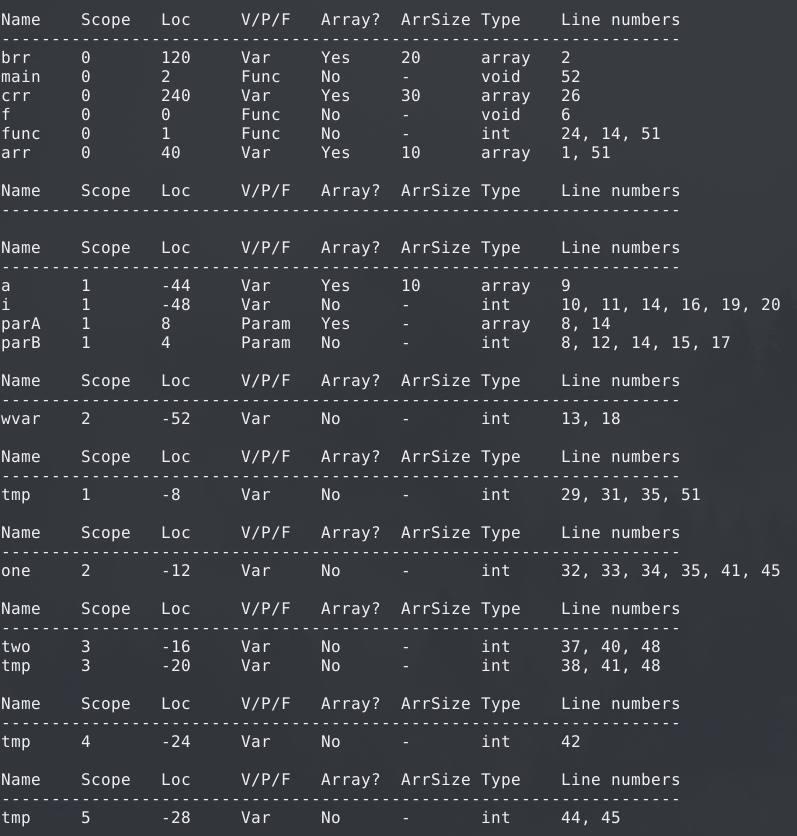
\includegraphics[width=\linewidth]{testresult.png}
\caption{Output}
\label{fig:output}
\end{figure}

또한 Semantic Error처리 확인을 위해 16개의 서로 다른 에러가 나오는 테스트 파일을 만들어 Julia 언어로 Coverage를 테스트하는 스크립트를 만들어 테스트하였다.

\section{기타}

\subsection{연구 조원 기여도}

\begin{itemize}
	\item 김규래: 50\%
	\item 박건: 50\%
\end{itemize}

\subsection{자체 평가}

Symbol table을 Global로 처리하지 않고, Opaque pointer \texttt{SymTable}핸들로 관리하여 메모리 누수를 방지하고 reentrancy를 보존하였다.

\subsection{느낀 점}

이번 프로젝트에서는 변수의 가능한 타입이 \texttt{int}밖에 없어서 Semantic Analysis가 간단했지만, 여러 타입이 추가되면 훨씬 어려워질 것이라는 생각이 들었다.

\end{document}